\documentclass[article,12pt,onesidea,4paper,english,brazil]{abntex2}

\usepackage{lmodern, indentfirst, nomencl, color, graphicx, microtype, lipsum, textcomp}		
\usepackage[T1]{fontenc}		
\usepackage[utf8]{inputenc}		

\setlrmarginsandblock{2cm}{2cm}{*}
\setulmarginsandblock{2cm}{2cm}{*}
\checkandfixthelayout

\setlength{\parindent}{1.3cm}
\setlength{\parskip}{0.2cm}

\SingleSpacing

\begin{document}
	
	\selectlanguage{brazil}
	
	\frenchspacing 
	
	\begin{center}
		\LARGE BIOPROSPECÇÃO DE \textit{RALSTONIA SOLANACEARUM}: IDENTIFICAÇÃO AVALIAÇÃO DA ATIVIDADE ANTIMICROBIAL DE MICRORGANISMOS ENDOFÍTICOS
		
		\normalsize
Mateus Barbizan\footnote{Bolsista (PIBITI - IFRO), tccmateusbarbizan@gmail.com, Campus Colorado do Oeste. } 
Daniela Barbizan\footnote{Bolsista (PIBIC EM - CNPq), bdaaniela@gmail.com, Campus Colorado do Oeste.} 
		Odair Antonio Barbizan\footnote{Orientador, odair.barbizan@ifro.edu.br, Campus Colorado do Oeste} \\
		Nélio Ferreira\footnote{Co-orientador(a), nelio.ferreira@ifro.edu.br, Campus Colorado do Oeste.} 
		Raniele Ferreira de Paula
	\end{center}
	
	% resumo em português
	\begin{resumoumacoluna}
		Com o objetivo de explorar as comunidades de microrganismos endofíticos de tomateiros visando à identificação e seleção de microrganismos com atividade antimicrobiana contra patógenos de interesse na indústria alimentícia e agronômico, o presente projeto utilizou a metodologia de bioprospecção, que consiste em selecionar plantas que em meio à cultura infestada pelo patógeno \textit{ralstonia solanacearum} que apresentam resistência à doença. Após os microorganismos serem isolados os mesmos foram utilizados em bioensaios com discos de difusão conforme procedimentos definidos por Huang et al. (2001). O resultado final consistiu na identificação e cultivo da \textit{ralstonia solanacearum} em meio de cultura seletivo adaptado, e, com o teste de bio ensaio constatamos atividade antibiótica no solo isolado das plantas no entorno da plantação dos tomateiros.
		\vspace{\onelineskip}
		
		\noindent
		\textbf{Palavras-chave}:bioprospecção, bioensaio, formação acadêmica.
	\end{resumoumacoluna}
	
	\textual
	
	\section*{Introdução}
	
A procura e descoberta de um fenômeno biológico que possa ser explorado é o passo inicial em um projeto biotecnológico, no entanto tão crucial quanto qualquer outra etapa neste processo (Bull et al., 1992). A biotecnologia é baseada na busca e descoberta de recursos biológicos industrialmente exploráveis. Uma abordagem clássica das etapas do processo de busca e descoberta biotecnológica passa resumidamente pela coleta de material biológico adequado, seguida da seleção e triagem de materiais com os atributos desejados, seleção final do(s) melhor(es) candidato(s) a partir de uma lista reduzida de opções, e culmina com o desenvolvimento de um produto comercial ou processo industrial (Bull et al, 2000). O objetivo principal do projeto foi explorar as comunidades de microrganismos endofíticos de tomateiros visando à identificação e seleção de microrganismos com atividade antimicrobiana contra o patógeno \textit{ralstonia solanacearum} de interesse na indústria alimentícia, agronômica e na formação acadêmica do profissional ligado a agricultura.
	
	\section*{Material e Método}
	
O material vegetal (tomateiros) foi coletado das estufas do assentamento conhecido como Agrovila de Vilhena/RO região de ocorrência das patologias causadas pela bactéria \textit{ralstonia solanacearum}.  Em cada coleta foi obtido material de quatro plantas independentes distribuídas dentro da região de coleta. De cada planta foi retirada aleatoriamente amostras visivelmente infectadas. As amostras foram embaladas em sacos plásticos e levadas para o Laboratório de Biologia onde ocorreu o isolamento dos microrganismos endofíticos no mesmo dia. Após a desinfecção das amostras vegetais para o isolamento de microrganismos endofíticos foi necessário que a superfície do material vegetal fosse desinfetada para retirada de microrganismos epifíticos e contaminantes. Os procedimentos de desinfecção do material vegetal e isolamento de microrganismos endofíticos foram realizados conforme descrito por Araújo e colaboradores (2000). Para desinfecção, as amostras sadias de tecidos vegetais sofreram uma série de lavagens sequenciais com etanol 70\% (30 segundos), hipoclorito de sódio 3\% (3 minutos), etanol 70\% (30 segundos) e duas vezes com água destilada esterilizada (6 minutos) (Araújo et. al., 2000). A eficiência da desinfecção do material vegetal foi avaliada pelo plaqueamento em meio ágar-batata-dextrose (BDA) e TSA de alíquotas da água utilizada na última lavagem do material vegetal e pelo pressionamento dos fragmentos desinfestados sobre o meio de cultura (Araújo et. al.,2000).

Para o isolamento de bactérias endofíticas, 1 g das amostras vegetais desinfetadas superficialmente foram maceradas em 9 ml de solução salina (0.85\%) estéril. A suspensão obtida foi diluída serialmente e alíquotas de 0.1 ml de cada diluição sendo plaqueadas em meio sólido TSA contendo 50 mg/ml do antifúngico benomil. As placas inoculadas foram incubadas a 28°C por até 10 dias, sendo o crescimento dos microrganismos acompanhado diariamente. Após, as colônias crescidas nas placas foram contadas para determinação do número de unidades formadoras de colônia (UFC). A densidade da população de bactérias endofíticos foi estimada pelo peso fresco e pelo fator de diluição. As diferentes colônias crescidas foram repicadas e transferidas para meio TSA sem antifúngico para purificação do isolado. As bactérias isoladas foram armazenadas em meio sólido TSA inclinado a 4°C e em glicerol 30\%.

A avaliação da atividade antimicrobiana foi feita pelo bioensaio de disco de difusão conforme procedimentos definidos por Huang et al. (2001). A suspensão (105 unidades formadoras de colônias (UFC)/ml) de células (ou esporos) de bactérias, leveduras ou fungos foi espalhada na superfície do meio de cultura BDA. Discos de papel estéreis (Whatman) foram impregnados com o caldo de fermentação e então, posicionados na superfície do meio de cultura inoculado. No controle negativo foi inoculado o meio de cultura e no controle positivo foi utilizado
30 $\mu$g/ml cloramfenicol para bactérias e 30 $\mu$g/ml cetoconazol para fungos e leveduras. As placas foram incubadas a 28°C por 2-5 dias. Após crescimento, a atividade antimicrobiana foi avaliada pelo diâmetro do halo de inibição (em mm) ao redor do disco de papel.
	
	\section*{Resultados e Discussão}

Segundo a literatura consultada a tarefa mais complicada é separar as murchas bacteriana, de fusário e de verticílio. Neste caso a EMBRAPA, recomenda em seus trabalhos técnicos o procedimento do teste do copo. Este foi realizado cortando-se uma pequena porção (cerca de 5 cm) da parte mais inferior do caule de planta doente, colocou-se em seguida ligeiramente submersa em frasco transparente com água limpa (Figura 1). A presença de um filete leitoso saindo do tecido em direção ao fundo do copo indica	a	presença		da	murcha-bacteriana.		A complementação	do	diagnóstico	foi	realizada	em laboratório: colônias típicas de R. solanacearum (Figuras 2 (A) e (B)) obtidas a partir da suspensão do exsudado leitoso e cultivado em meios de cultura diferencial de Kelman (1954).

\begin{figure}[h]
	\centering
	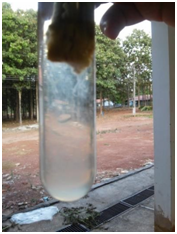
\includegraphics[width=0.3\linewidth]{pip06.png}
	\caption{Testedocopo,mostrando exsudaçãodepusbacterianoem cauledetomateiroafetadopela murchabacteriana.}
	\label{fig:Rotulo}
\end{figure}

\begin{figure}[h]
	\centering
	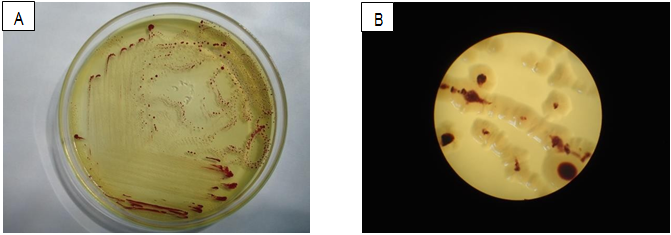
\includegraphics[width=0.7\linewidth]{pipi.png}
	\caption{(A) Colônias de Ralstonia solanacearume mmeiodeKelman comtetrazólio. (B) Aumento de 40x destacandoo tetrazólio interagindo com o núcleo.}
\end{figure}

Após o isolamento, cultivo e identificação das bactérias através da reação com o tetrazólio, conforme protocolo da EMBRAPA, foi realizado o teste de inibição com o sobrenadante das lavagens efetuadas nas amostras. Conforme podemos perceber na figura 3, houve inibição do crescimento das bactérias na área ao redor dos discos, indicando a presença de organismos ou substancias inibidoras de crescimento no solo e raízes de plantas sadias coletadas nas estufas do Instituto Federal de Rondônia – IFRO.
	
	\section*{Conclusões}
		
	Concluímos que o objetivo principal do projeto de explorar as comunidades de microrganismos endofíticos de tomateiros visando à identificação e seleção de microrganismos com atividade antimicrobiana contra o patógeno \textit{Ralstonia Solanacearum} foi atingido, pois conseguimos identificar a presença da bactéria causadora da doença conhecida como murcha. Identificamos a presença de organismos e ou substâncias com características inibidoras de crescimento bacteriano nos discos de inibição. Tornando-se o próximo passo para a continuidade do projeto com a possível identificação desta inibição
	
	\begin{figure}[h]
		\centering
		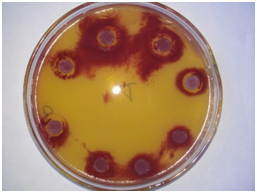
\includegraphics[width=0.7\linewidth]{pip1.png}
		\caption{Presença de halos de inibição,indicando presença de organismos/substâncias inibidoras de crescimento bacteriano.}
	\end{figure}
	
	\section*{Agradecimentos}
	
	Gostaríamos de agradecer ao Professor Dr. Marcos Aurelio Anequine Macedo pela ajuda nas coletas, transporte e identificação das plantas utilizadas.
	
	\section*{Instituição de Fomento}
	
	Ao Instituto Federal de Educação, Ciência e Tecnologia de Rondônia - IFRO que conta com apoio financeiro do Conselho Nacional de Desenvolvimento Científico e Tecnológico (CNPq) que fomentaram a realização da pesquisa, seja com concessão de auxílio(s) ou bolsa(s).
	
	\sloppy
	\section*{Referências}
	
	\noindent ARAÚJO, W.L.; MACCHERONI JR., W.; AGUILAR-VILDOSO, C.I.; BARROSO, P.A.V. SARIDAKIS, H.O.; AZEVEDO, J.L. Variability and interactions between endophytic bacteria and fungi isolated from leaf tissues of citrus rootstocks. Can. J. Microbiol., v.47, p.229-236, 2001. DOI: 10.1139/cjm-47-3-229.

	\noindent BULL, A.T.; GOODFELLOW, M.; SLATER, J.H. Biodiversity as a  source  of innovation in biotechnology. Annual Review of Microbiology, v. 46, p.219-252,1992.
	
	\noindent BULL, A.T.; WARD, A.C.; GOODFELLOW, M. Search and discovery strategies for biotechnology: the paradigm shift. Microbiology  and  Molecular  Biology  Reviews,  v.64, p.573-606,2000.
	
	\noindent CRAWFORD, D. L., J. M. LYNCH, J. M. WHIPPS, AND M. A. OUSLEY. Isolation and
	characterization of actinomycete antagonists of a fungal root pathogen. Appl. Environ. Microbiol., v. 59, p.3899-3905, 1993.
	
	\noindent GUNATILAKA, L.A.A. Natural Products from Plant-Associated Microorganisms: Distribution, Structural Diversity, Bioactivity,  and  Implications  of  Their Occurrence. J. Nat. Prod., v. 69, p.509-526,2006.
	
	\noindent HUANG,Y.; WANG, J.; LI, G.; ZHENG, Z.; SU, W. Antitumor  and  antifungal  activities in endophytic fungi isolated from pharmaceutical plants Taxus mairei, Cephalataxus fortunei and Torreya grandis. FEMS Immunology and Medical Microbiology, v. 31, p.163-167, 2001.
	
	\noindent HUNTER-CEVERA,   J.C.   The   value    of    microbial   diversity.    Current    Opinion in Microbiology, v. 1, p.278-285,1998.
	
	\noindent PINTO, A.C.; SILVA, D.H.S.; BOLDANI, V.S.; LOPES, N.P. Produtos naturais: Atualidade, desafios e perspectivas. Química Nova, v. 25, n. 1, p.45-61, 2002.
	
	\noindent QIN, S.; XING, K.; JIANG, J.; XU, L.; LI, W. Biodiversity, bioactive natural products and biotechnological potential of plant-associated endophytic actinobacteria. Appl Microbiol. Biotechnol., v. 89, p.457-473, 2011. DOI: 10.1007/s00253-010-2923-6.
	
	\noindent SANTOS, R.I. Metabolismo básico e origem dos metabolismos secundários. In: SIMÕES, C.M.O.; SCHENKEL, E.P.; GOSMANN, G.; MELLO, J.C.P.; MENTZ, L.A.\&
	
	
\end{document}